\documentclass[a4paper]{article}
\usepackage[margin=1in]{geometry}
\linespread{1.2}
%\overfullrule=2cm % for debugging purposes! comment in production
% displays overfill rule on side of the document

\usepackage[utf8]{inputenc}
\usepackage[english,polish]{babel}

% babel defines \lll
\let\babellll\lll
\let\lll\relax

\usepackage[htt]{hyphenat}
\usepackage{amsmath}
\usepackage{amssymb}
\usepackage{amsthm}
\usepackage{blindtext}
\usepackage{enumerate}
\usepackage{enumitem}
\usepackage{graphicx}
\usepackage{mathtools}
\usepackage{multicol}
\usepackage{polski}
%\usepackage[T1]{fontenc}
%\usepackage[scaled]{beramono}
\usepackage{hyperref}

\usepackage{color}
\definecolor{bluekeywords}{rgb}{0.13,0.13,1}
\definecolor{greencomments}{rgb}{0,0.5,0}
\definecolor{redstrings}{rgb}{0.9,0,0}

\usepackage{listings}
\lstset{language=[Sharp]C,
	showspaces=false,
	showtabs=false,
	breaklines=false,
	showstringspaces=false,
	breakatwhitespace=true,
	escapeinside={(*@}{@*)},
	commentstyle=\color{greencomments},
	%keywordstyle=\color{bluekeywords}\bfseries,
	stringstyle=\color{redstrings},
	basicstyle=\ttfamily
}


\title{Wstęp do Algorytmów Ewolucyjnych \\
	\large Raport z testów}

\date{\today}
\author{Kacper Sarnacki \and Monika Żurkowska}

\begin{document}
\maketitle

\section{Przypomnienie}
Celem naszego projektu było zaimplementowanie zmodyfikowanego algorytmu ewolucji różnicowej, w którym jako pierwszy z 3 punktów stosowanych podczas mutacji wybierana była średnia punktów populacji a następnie porównanie tego rozwiązanie z klasycznym algorytmem ewolucji różnicowej wykorzystując benchmark ''cec2013'' do testowania.

\section{Lista zmian}
W związku z długim czasem wykonywania się testów zmuszeni byliśmy przyjąć kilka poprawek w stosunku do przyjętych założeń ze Specyfikacji Wstępnej:

\begin{itemize}
\item Rozmiar wektorów dla których przeprowadziliśmy testy: 5 oraz 10
\item Mniejsza liczba kombinacji współczynników F i Cr (patrz \ref{sec:testy})
\item Liczba iteracji dla każdego testu: 10
\item  Algorytm porównujemy wyłącznie z klasycznym algorytmem z losowym doborem 3 punktów w przeciwieństwie do wcześniejszego założenia o porównaniu go z algorytmem losowym i algorytmem, w którym jako pierwszy z trzech punktów wybierany jest najlepszy spośród obecnej populacji
\item W warunku stopu dla algorytmów brana była pod uwagę liczba wywołań funkcji ewaluacyjnej zamiast - jak wcześniej założono - liczby iteracji.
\end{itemize}

\section{Testy}
\label{sec:testy}

Zgodnie z wymaganiami, nasze testy przeprowadziliśmy na benchmarku ''cec2013' dla naszego algorytmu oraz dla algorytmu klasycznego. Wyniki przedstawione zostały w tabelach poniżej.

\begin{figure}
\centering
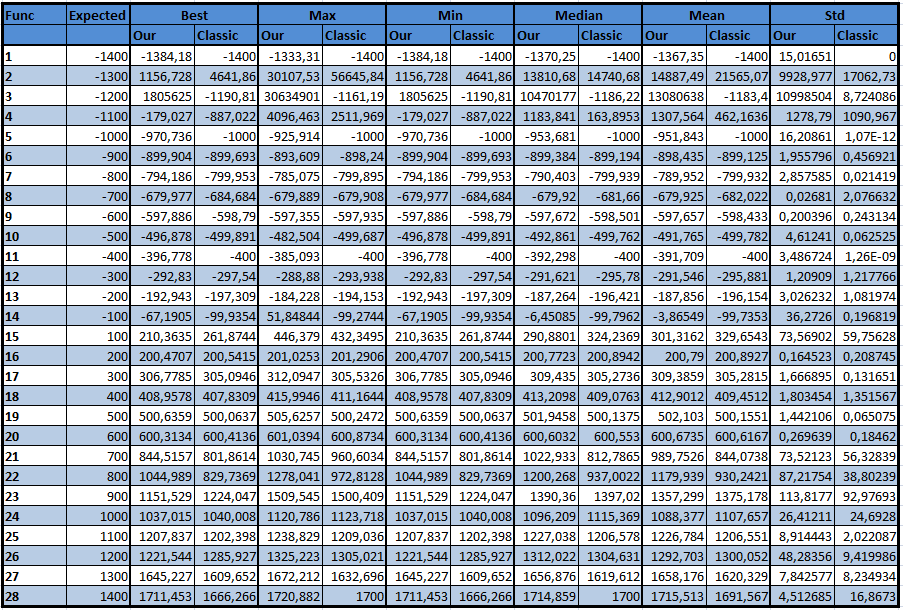
\includegraphics[width=\textwidth]{F25Cr25L5tab.png}
\caption{5-wymiarowa populacja. Wyniki dla parametrów: F = 0.25, Cr = 0.25}
\end{figure}

\begin{figure}
\centering
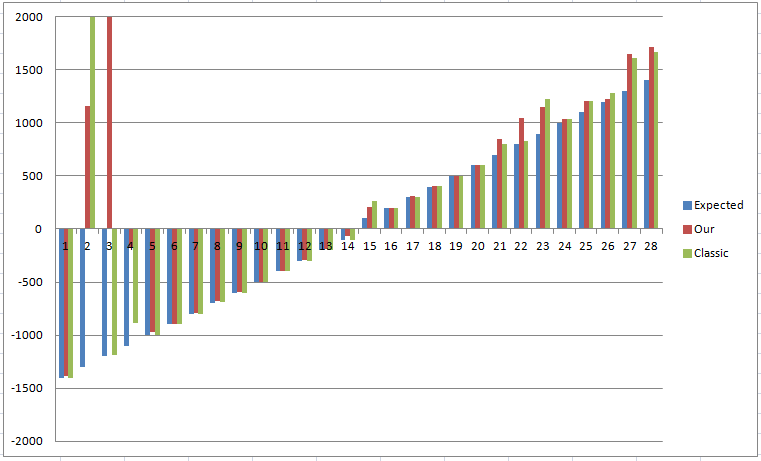
\includegraphics[width=\textwidth]{F25Cr25L5chart.png}
\caption{5-wymiarowa populacja. Wykres porównujący najlepsze rozwiązania dla naszego algorytmu oraz klasycznego. Parametry: F = 0.25, Cr = 0.25}
\end{figure}

\begin{figure}
\centering
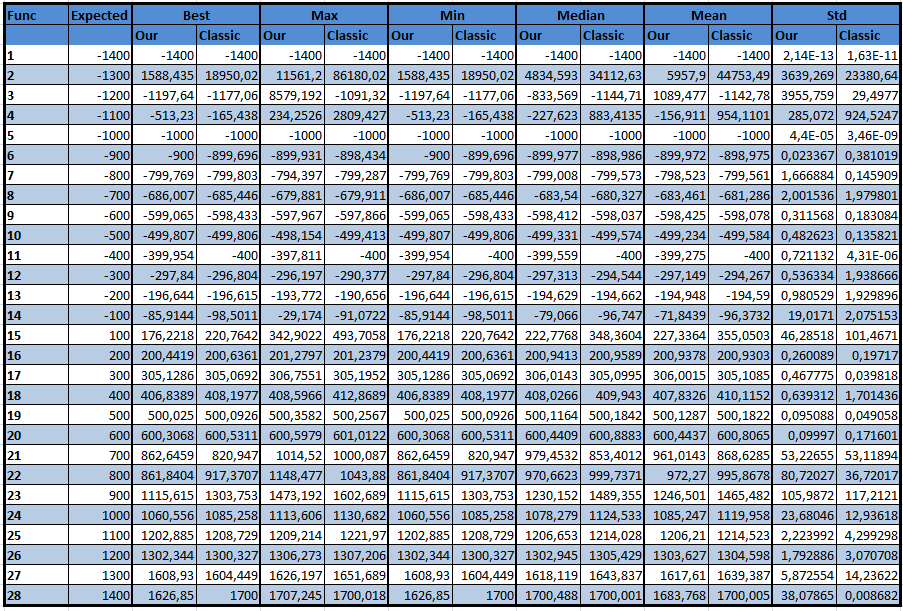
\includegraphics[width=\textwidth]{F5Cr25L5tab.png}
\caption{5-wymiarowa populacja. Wyniki dla parametrów: F = 0.5, Cr = 0.25}
\end{figure}

\begin{figure}
\centering
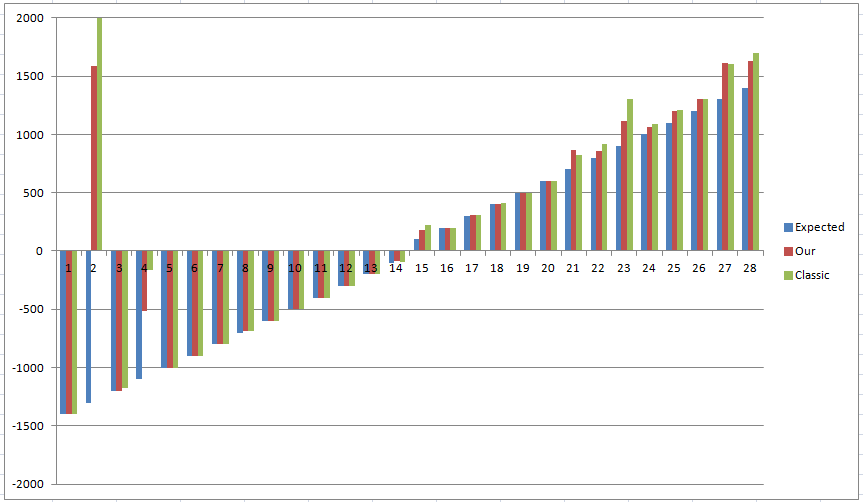
\includegraphics[width=\textwidth]{F5Cr25L5chart.png}
\caption{5-wymiarowa populacja. Wykres porównujący najlepsze rozwiązania dla naszego algorytmu oraz klasycznego. Parametry: F = 0.5, Cr = 0.25}
\end{figure}

\begin{figure}
\centering
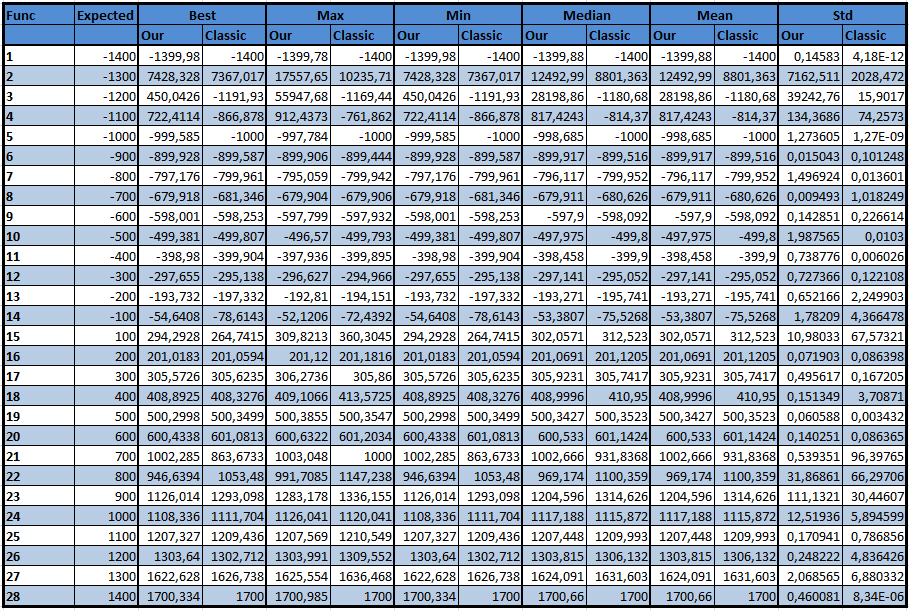
\includegraphics[width=\textwidth]{F5Cr5L5tab.png}
\caption{5-wymiarowa populacja. Wyniki dla parametrów: F = 0.5, Cr = 0.5}
\end{figure}

\begin{figure}
\centering
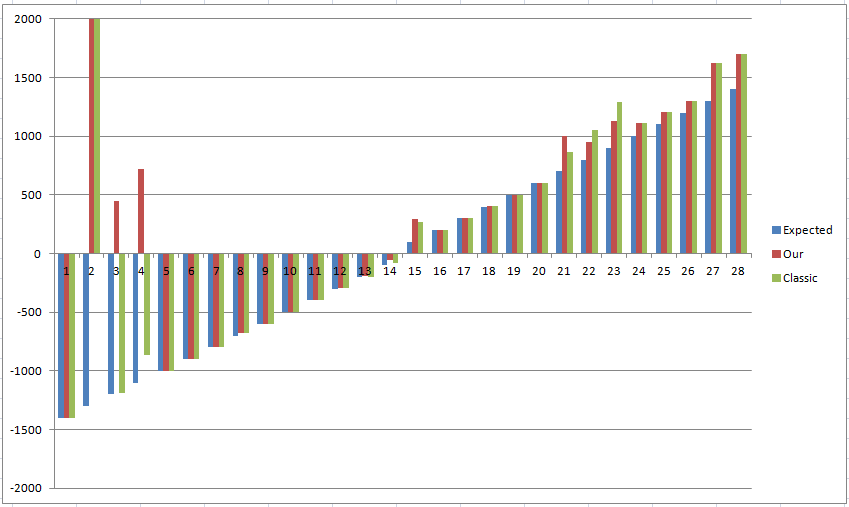
\includegraphics[width=\textwidth]{F5Cr5L5chart.png}
\caption{5-wymiarowa populacja. Wykres porównujący najlepsze rozwiązania dla naszego algorytmu oraz klasycznego. Parametry: F = 0.5, Cr = 0.5}
\end{figure}

\begin{figure}
\centering
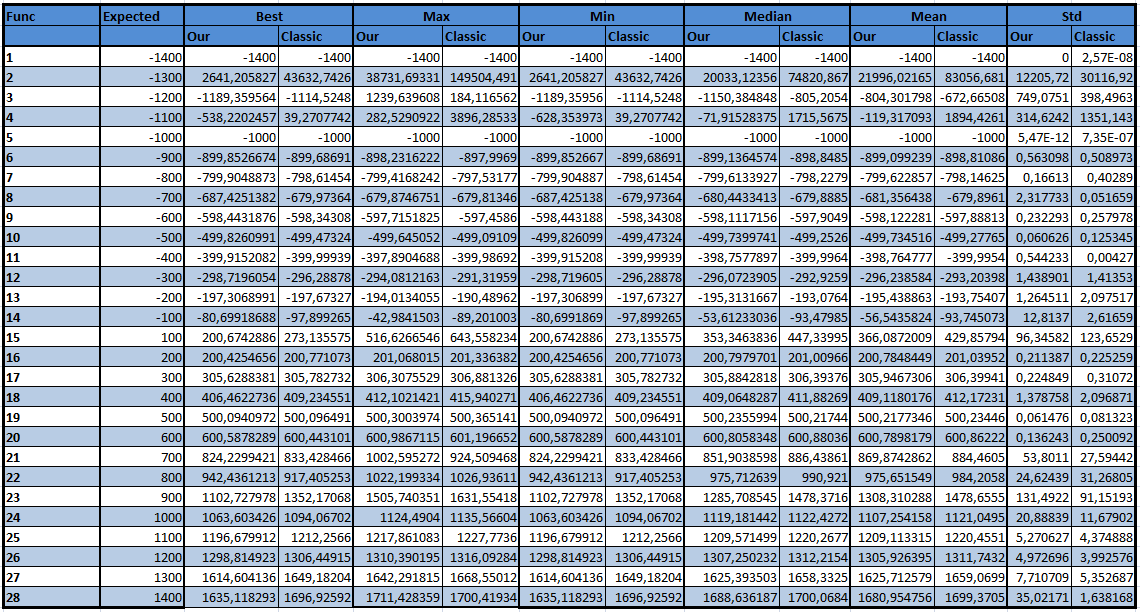
\includegraphics[width=\textwidth]{F75Cr25L5tab.png}
\caption{5-wymiarowa populacja. Wyniki dla parametrów: F = 0.75, Cr = 0.25}
\end{figure}

\begin{figure}
\centering
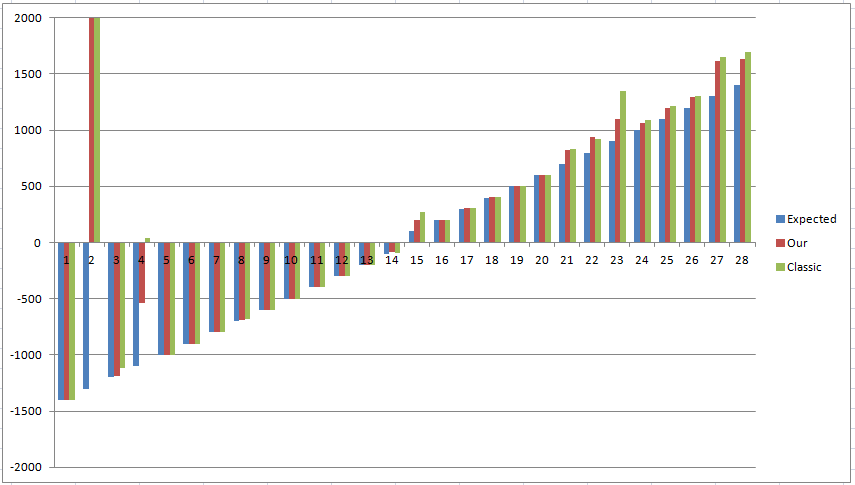
\includegraphics[width=\textwidth]{F75Cr25L5chart.png}
\caption{5-wymiarowa populacja. Wykres porównujący najlepsze rozwiązania dla naszego algorytmu oraz klasycznego. Parametry: F = 0.75, Cr = 0.25}
\end{figure}

\begin{figure}
\centering
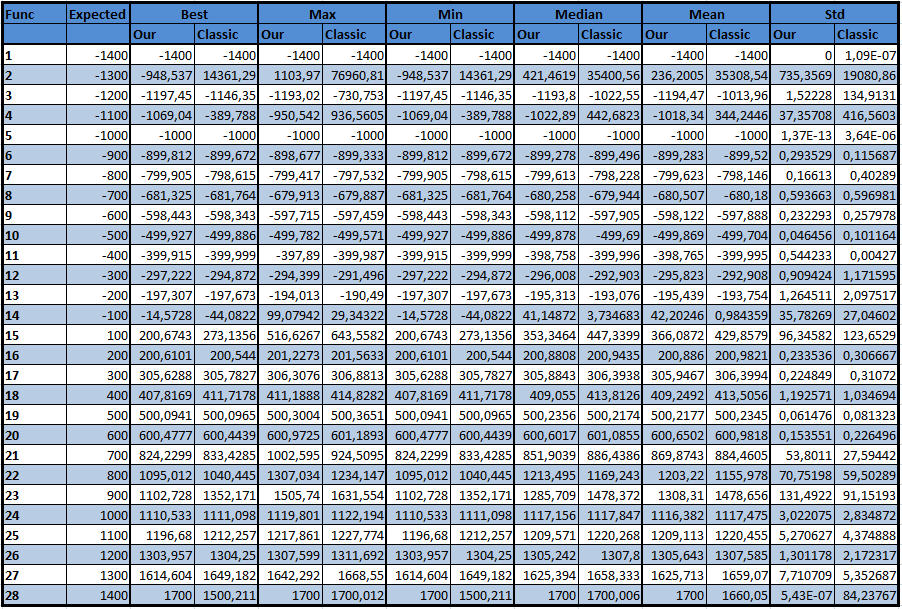
\includegraphics[width=\textwidth]{F75Cr5L5tab.png}
\caption{5-wymiarowa populacja. Wyniki dla parametrów: F = 0.75, Cr = 0.5}
\end{figure}

\begin{figure}
\centering
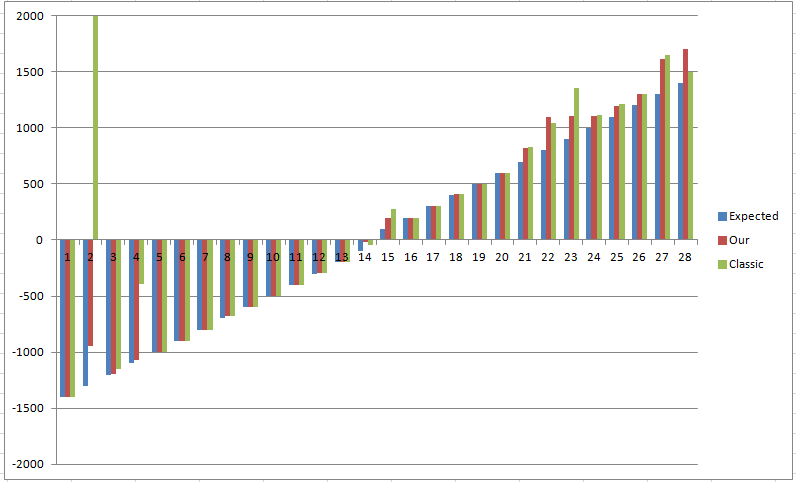
\includegraphics[width=\textwidth]{F75Cr5L5chart.png}
\caption{5-wymiarowa populacja. Wykres porównujący najlepsze rozwiązania dla naszego algorytmu oraz klasycznego. Parametry: F = 0.75, Cr = 0.5}
\end{figure}

\begin{figure}
\centering
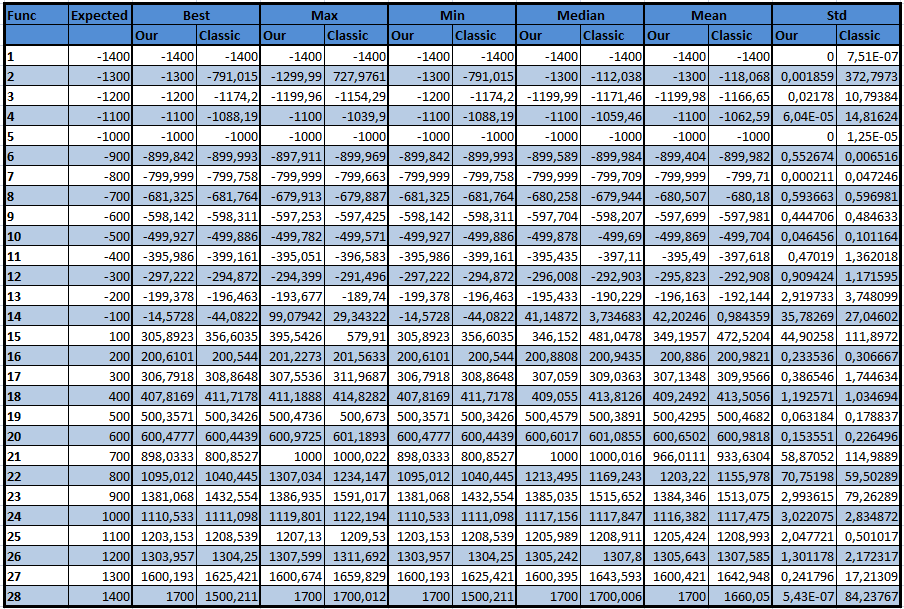
\includegraphics[width=\textwidth]{F75Cr75L5tab.png}
\caption{5-wymiarowa populacja. Wyniki dla parametrów: F = 0.75, Cr = 0.75}
\end{figure}

\begin{figure}
\centering
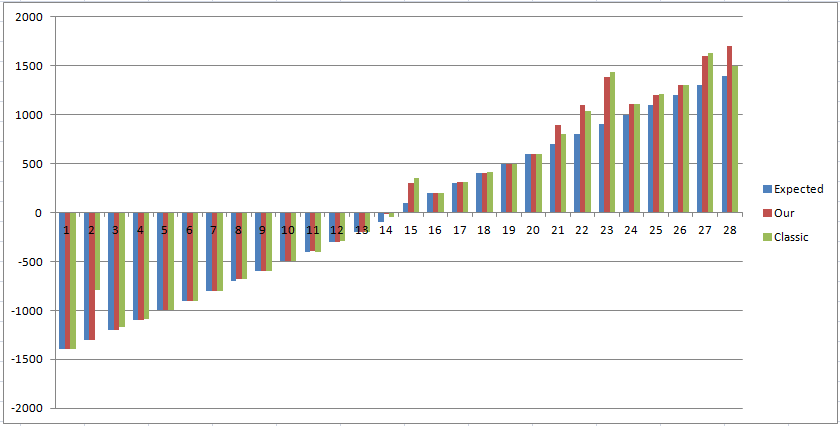
\includegraphics[width=\textwidth]{F75Cr75L5chart.png}
\caption{5-wymiarowa populacja. Wykres porównujący najlepsze rozwiązania dla naszego algorytmu oraz klasycznego. Parametry: F = 0.75, Cr = 0.75}
\end{figure}

\begin{figure}
\centering
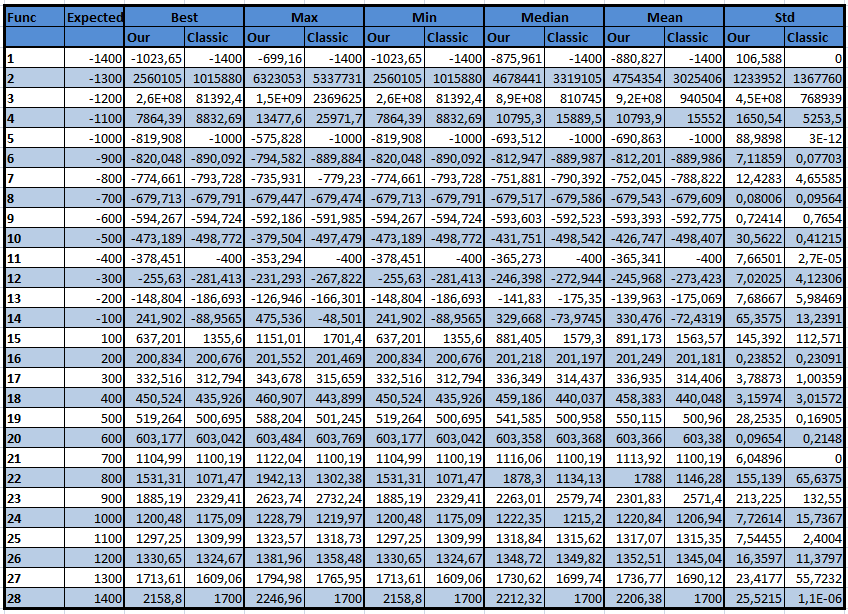
\includegraphics[width=\textwidth]{F25Cr25L10tab.png}
\caption{10-wymiarowa populacja. Wyniki dla parametrów: F = 0.25, Cr = 0.25}
\end{figure}

\begin{figure}
\centering
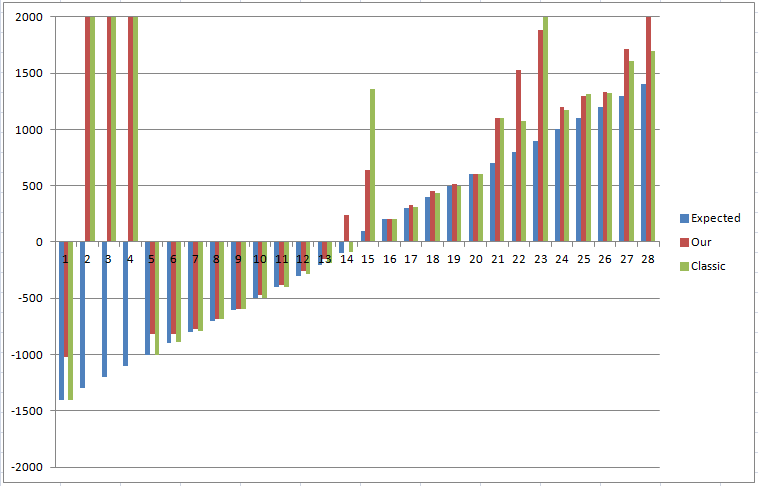
\includegraphics[width=\textwidth]{F25Cr25L10chart.png}
\caption{10-wymiarowa populacja. Wykres porównujący najlepsze rozwiązania dla naszego algorytmu oraz klasycznego. Parametry: F = 0.25, Cr = 0.25}
\end{figure}

\begin{figure}
\centering
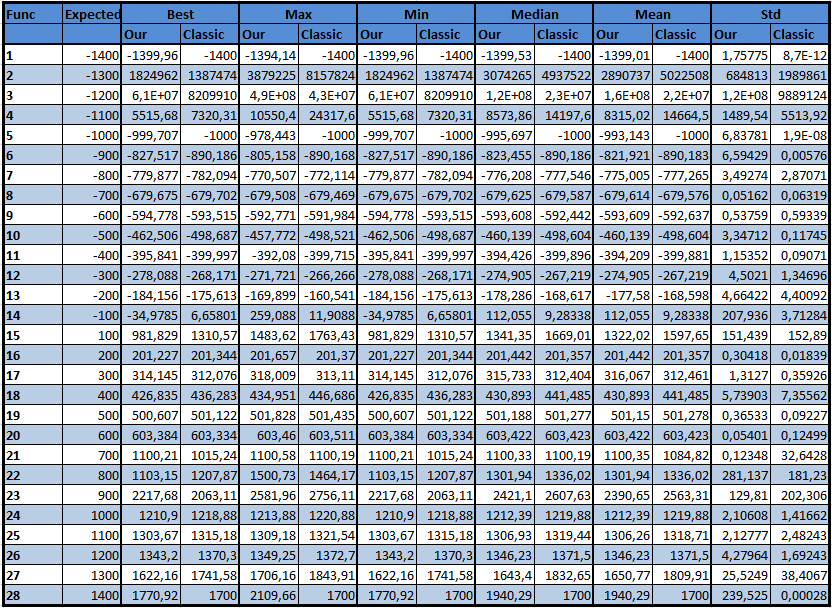
\includegraphics[width=\textwidth]{F5Cr25L10tab.png}
\caption{10-wymiarowa populacja. Wyniki dla parametrów: F = 0.5, Cr = 0.25}
\end{figure}

\begin{figure}
\centering
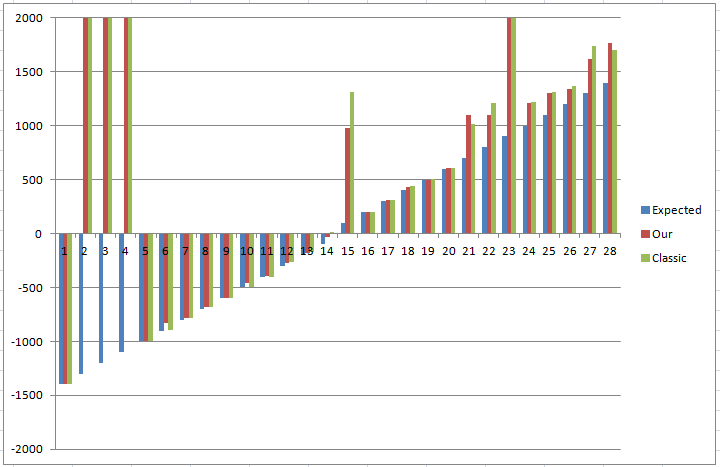
\includegraphics[width=\textwidth]{F5Cr25L10chart.png}
\caption{10-wymiarowa populacja. Wykres porównujący najlepsze rozwiązania dla naszego algorytmu oraz klasycznego. Parametry: F = 0.5, Cr = 0.25}
\end{figure}

\begin{figure}
\centering
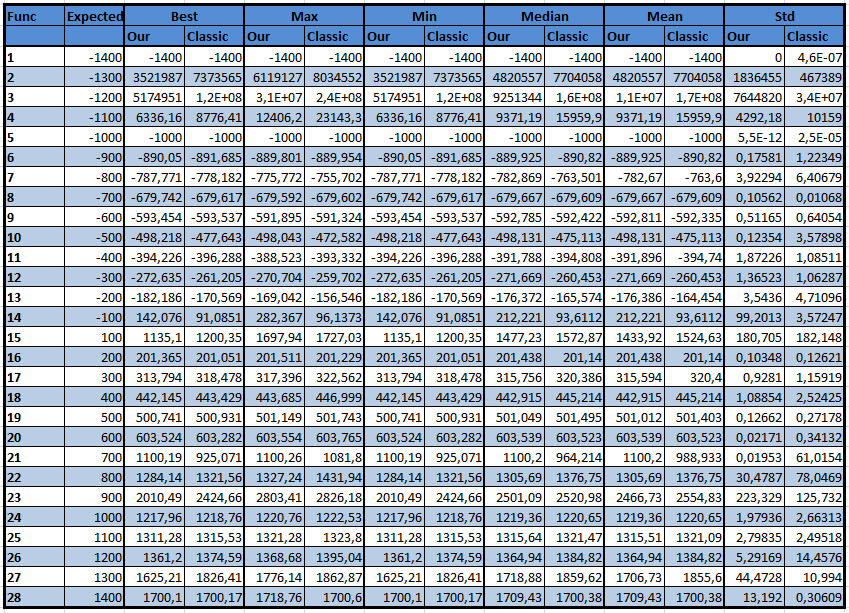
\includegraphics[width=\textwidth]{F75Cr25L10tab.png}
\caption{10-wymiarowa populacja. Wyniki dla parametrów: F = 0.75, Cr = 0.25}
\end{figure}

\begin{figure}
\centering
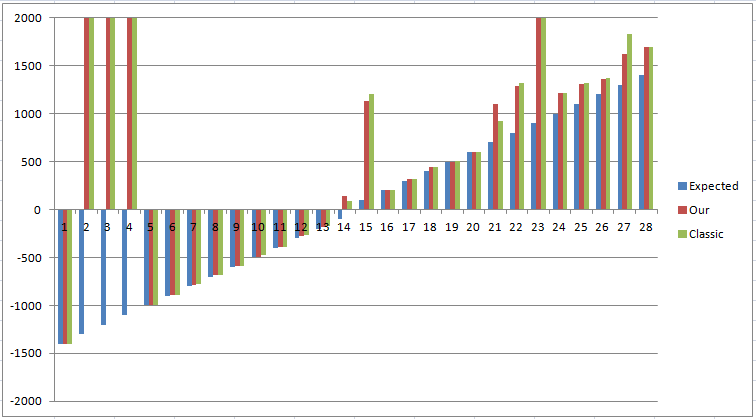
\includegraphics[width=\textwidth]{F75Cr25L10chart.png}
\caption{10-wymiarowa populacja. Wykres porównujący najlepsze rozwiązania dla naszego algorytmu oraz klasycznego. Parametry: F = 0.75, Cr = 0.25}
\end{figure}

\begin{figure}
\centering
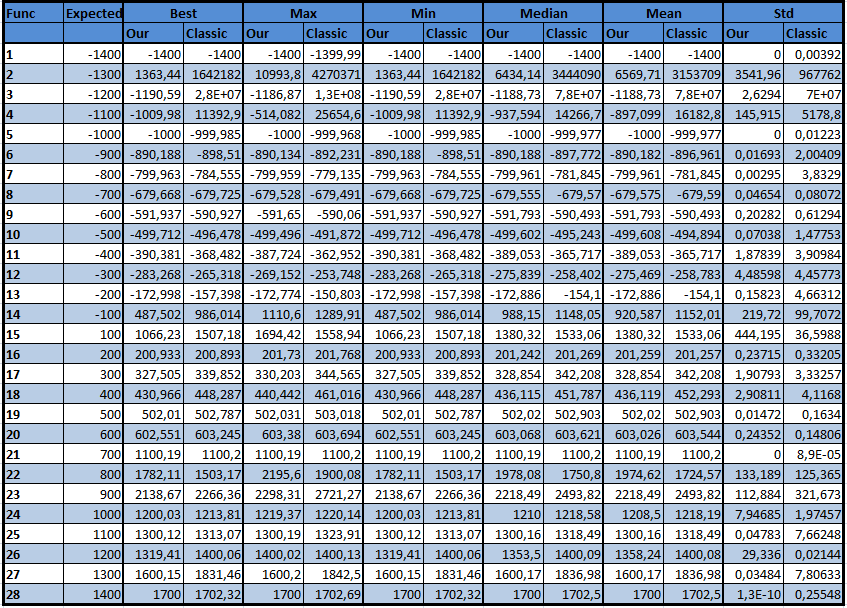
\includegraphics[width=\textwidth]{F75Cr75L10tab.png}
\caption{10-wymiarowa populacja. Wyniki dla parametrów: F = 0.75, Cr = 0.75}
\end{figure}

\begin{figure}
\centering
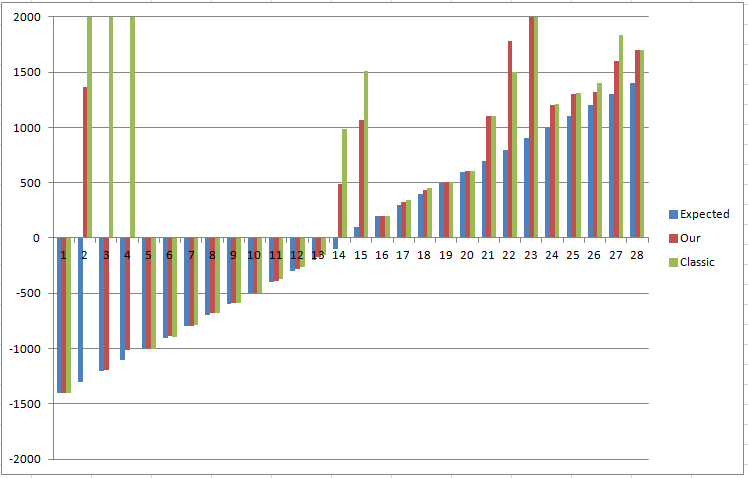
\includegraphics[width=\textwidth]{F75Cr75L10chart.png}
\caption{10-wymiarowa populacja. Wykres porównujący najlepsze rozwiązania dla naszego algorytmu oraz klasycznego. Parametry: F = 0.75, Cr = 0.75}
\end{figure}

\end{document}

